\documentclass[a4paper]{article}

\usepackage[a4paper,top=0.4in,left=0.4in,right=0.4in,bottom=0.4in]{geometry}
\usepackage{graphicx}
\usepackage{rotating}


\usepackage{setspace}
\usepackage{float}
\graphicspath{ {./images/} }

\usepackage{tabularx,ragged2e,booktabs,caption}
\newcolumntype{C}[1]{>{\Centering}m{#1}}
\renewcommand\tabularxcolumn[1]{C{#1}}

\usepackage{titling}
\setlength{\droptitle}{-10em}

\title{Group Project - 7CCSMGPR \hspace{0.5 cm}Deadline Fighters}
\renewcommand\maketitlehookc{\vspace{-10ex}}

\begin{document}

{\setstretch{0.75}
\begin{center}
		\LARGE{Group Project - 7CCSMGPR}
\end{center}
\begin{center}
		\hspace{0.5cm} Deadline Fighters \hspace{0.5 cm} Final report - March 24, 2019
\end{center}


\section{Desktop client implementation}
We made a planning framework when we realized the functionality of the desktop client. We firstly mapped out implementing upload files, download files, delete files, rename files, edit files and other functions. Secondly, implementing the ability to combine available functions into one file synchronization feature. Finally, we will beautify the interface and improve user experience.\\\\
In the process of implementation, the main process is divided into the following steps:\\\\




\begin{minipage}{\linewidth}
\centering
\captionof{table}{Steps of processes} \label{table:conflict}
\begin{tabular}[H]{|C{0.75cm}|C{10.5cm}|}\toprule[1.5pt]
\bf Step & \bf Process \\\midrule
1 	&  \begin{flushleft}Configure the computer to connect to AWS S3.\end{flushleft}\\\hline
2   &  \begin{flushleft}Create a new electron project.\end{flushleft}\\\hline
3   &  \begin{flushleft}Open the project, configure the Access key ID and Secret Access Key in code and make the project connect to S3.\end{flushleft}\\\hline
4   &  \begin{flushleft}Add a file selector and initially implement the function of uploading a single file to S3.\end{flushleft}\\\hline
5  	&  \begin{flushleft}Initial download of a file with a specific name.\end{flushleft}\\\hline
6   &  \begin{flushleft}Preliminary deletion of files with specific names.\end{flushleft}\\\hline
7   &  \begin{flushleft}Rename the file on the desktop client and upload it to S3.\end{flushleft}\\\hline
8   &  \begin{flushleft}Try to use E-tag and MD5 to edit the file and incrementally upload the changed part. Then plan to compare the local file and the last modified time of the server file to upload the modified file, but it is not successful.\end{flushleft}\\\hline
9   &  \begin{flushleft}Create a folder called deadlinefighters on the local disk.\end{flushleft}\\\hline
10  &  \begin{flushleft}List all files stored on the server.\end{flushleft}\\\hline
11  &  \begin{flushleft}Add button function to every listed file.\end{flushleft}\\\hline
12  &  \begin{flushleft}Click on each individual file, jump out of the two dialogs, download and delete, and perform related operations for specific files.\end{flushleft}\\\hline
13  &  \begin{flushleft}Plan to simplify syncing, first upload all local files then download all server files.\end{flushleft}\\\hline
14  &  \begin{flushleft}Get a list of local files and use a loop to add an upload function to each file.\end{flushleft}\\\hline
15  &  \begin{flushleft}Get a list of server files and use a loop to add a download method to each file.\end{flushleft}\\\hline
16  &  \begin{flushleft}Add upload all function and download all function to the sync function click event.\end{flushleft}\\\hline
17  &  \begin{flushleft}Add CSS.\end{flushleft}\\
\bottomrule[1.25pt]
\end {tabular}\par
\bigskip
\end{minipage}

At the step 4, upload is the first function in file synchronization system that I tried to achieve, html5 had an input method that type = \emph{file}, it will generate a file selector and users can choose a file that in the local disk. I got the element of file in the scripts and put the element in parameters, the parameters that S3 need usually are file name, file type and file content, and file should be uploaded according to the desired format what S3 provided. S3 has an upload method and when desktop sends the parameters, the server will catch and return the error or upload file successfully.\\\\

At the next step, I firstly added a download function and that can download a special file, like \emph{1.txt}, from server to local. I used \emph{fs} module in node.js, the \emph{fs} module is the file system module, which is responsible for reading and writing files, it needs to introduce \emph{fs} module in code before use, like \emph{var fs = require(“fs”)}. I got the bucket (a storage system in S3) and key (file name) of a file, stored them in a parameter and passed it to \emph{getObject} function in S3 to got the whole element of file. Then I used \emph{fs.writeFileSync(filename, data, [options])}, filename will give a name of file and a path that where this file will be located. 

\begin{figure}[h!]
\centering
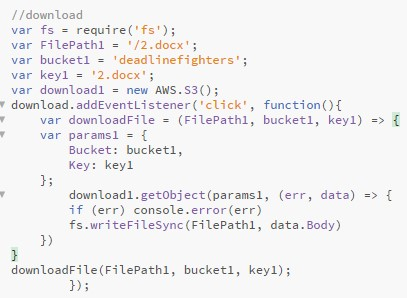
\includegraphics[scale=1.3]{code1}
\caption{download code}
\label{fig:code1}
\end{figure}

At the step 7, because S3 had no direct rename method, I only can copy a special file on the server first and give it a new name, then delete the original file.\\\\

As for \emph{edit} function, in our plan, we will handle edited files with delta synchronization. Delta sync is used to synchronize the modified portion of the file instead of re-uploading the entire file, in order to increase the speed of server processing. Delta sync relate to MD5 Algorithm and E-tag.But in the end \emph{edit} did not succeed.\\\\

Considering that the downloaded files need to be stored in a folder for users conveniently view, I tried to add a method to automatically create a folder in local. JavaScript is not allowed to access local files, but \emph{fs} module can help to deal with it. I used \emph{fs.mkdir} function to create a primary directory named \emph{deadlinefighters}.\\\\


In order to better displayed the files on the server, we designed to list all the files. I cited jQuery to simplify code, firstly, used \emph{listObjects} function which S3 was provided to list all the files in the backstage. Then, got the key (file name) and rendered it to the front-end interface. \emph{\$.each(objects, function(i, content)} is used for traversing the array, the array here is objects, which contained all the file contents, content represents each file, content.Key shows the name of each file.\\\\

\begin{figure}[h!]
\centering
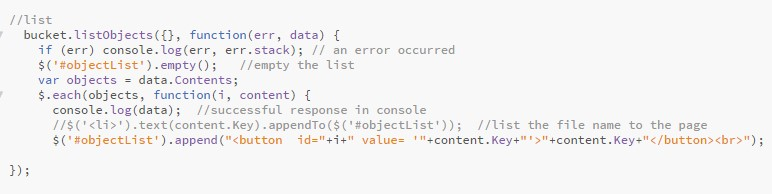
\includegraphics[scale=1.2]{code2}
\caption{download code}
\label{fig:code2}
\end{figure}

I changed each line of file to a button and that was convenient to add click events for download and delete functions later.\\\\
I set two dialogs to one file, one was download function, the other was delete function. The download function was similar with the previous code, key and file path need to be change, just passed the file values obtained by clicking the button to them. The file following represented key and got the corresponding file object from dialog, the file path pointed to the newly created folder.\\\\

\begin{center}
\emph{var file = \$(this).val();}\\\\
\emph{var filePath = '/deadlinefighters'+'/' + file;}
\end{center}

The delete function is something different, when the server file is deleted, the local file will be deleted too. Therefore, I added a loop algorithm to traverse local files for each deleted server file, when the name of the local file is equal to the name of the server file, the local file will also be deleted.

\begin{figure}[h!]
\centering
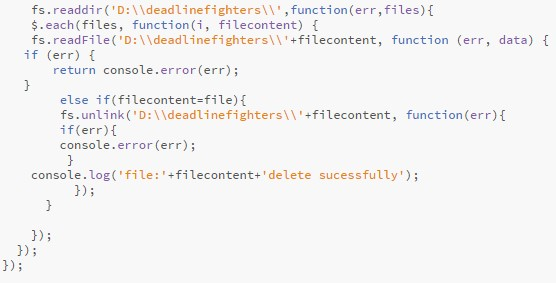
\includegraphics[scale=1.2]{code3}
\caption{download code}
\label{fig:code3}
\end{figure}

Because the files existed under a specific folder, it needed to first specify to the folder directory and then used the loop to get information about each file. At first, when read each file’s name, I didn’t add the \emph{“'D:$\backslash$$\backslash$deadlinefighters$\backslash$$\backslash$'+”} before\\\\

However, the result returned an error, \emph{filecontent} represented all the data in a file, not only a name, so it can’t compare with the file name in server.\\\\

The step 13 to 16 mainly completed a simple synchronization function. \emph{Upload all} and \emph{download all} functions were all involving loop. \emph{Upload all} was similar with \emph{delete}, just added an upload method to the file loop. \emph{Download all} was unlike with local file loop, the method used here is to loop through the server's files and add the download method.\\\\

In general, the desktop client of the file synchronization system has the following buttons and functions:\\\\


\begin{minipage}{\linewidth}
\centering
\captionof{table}{Buttons and functions} \label{table:conflict}
\begin{tabular}[H]{|C{2 cm}|C{9.5 cm}|}\toprule[1.5pt]
\bf Button & \bf Function \\\midrule
sync 	&  \begin{flushleft}\item{Upload all files from a local folder to server.}\item{Download all files from server to local folder.}\end{flushleft}\\\hline
upload   &  \begin{flushleft}Upload another one file from local to server.\end{flushleft}\\\hline
each line of file   &  \begin{flushleft}List each line of file in server.\end{flushleft}\\\hline
download   &  \begin{flushleft}Download one file.\end{flushleft}\\\hline
delete  	&  \begin{flushleft}Delete one file.\end{flushleft}\\

\bottomrule[1.25pt]
\end {tabular}\par
\bigskip
\end{minipage}




\medskip

\end{document}
